\documentclass{beamer}
%\usetheme{Berlin}
%\usetheme{Ilmenau}
%\usetheme{Dresden}
%\usetheme{Berkeley}
%\usetheme{Bergen}
%\usetheme{Boadilla}
%\usetheme{Copenhagen}
%\usetheme{Hannover}
%\usetheme{Luebeck}
%\usetheme{AnnArbor}
%\usetheme{Darmstadt}
%\usetheme{Frankfurt}
\usetheme{Madrid}%azulito-li;la
%\usetheme{Warsaw}%int
%\usetheme{Antibes}
%\usetheme{CambridgeUS}%rojo-gris
%\usetheme{Malmoe}
%\usetheme{PaloAlto}

\usepackage{graphicx}
\usepackage[utf8]{inputenc}
\usepackage[spanish]{babel}
\usepackage{url}
%\usepackage{beamerthemeshadow}
\usepackage{caption}


\hyphenation{}


%Arreglos en el footnote
\makeatletter
\setbeamertemplate{footline}
{
  \leavevmode%
  \hbox{%
  \begin{beamercolorbox}[wd=.333333\paperwidth,ht=2.25ex,dp=1ex,center]{author in head/foot}%
    \usebeamerfont{author in head/foot}\insertshortauthor
  \end{beamercolorbox}%
  \begin{beamercolorbox}[wd=.58\paperwidth,ht=2.25ex,dp=1ex,center]{title in head/foot}%
    \usebeamerfont{title in head/foot}\inserttitle
  \end{beamercolorbox}%
  \begin{beamercolorbox}[wd=.1\paperwidth,ht=2.25ex,dp=1ex,center]{date in head/foot}%
    \usebeamerfont{date in head/foot}\insertframenumber{} / \inserttotalframenumber\hspace*{2ex} 
  \end{beamercolorbox}}%
  \vskip0pt%
}
\makeatother

%Apagar el menu de presentacion
\setbeamertemplate{navigation symbols}{}%remove navigation symbols

%Bloques con sombras


\begin{document}
\title{Optimización de viajes compartidos en taxis utilizando algoritmos evolutivos}
\author[G. Fagúndez de los Reyes \and R. Massobrio]{Gabriel Fagúndez de los Reyes \and Renzo Massobrio} 
\institute[]{Facultad de Ingeniería,\\
Universidad de la República,\\
Montevideo, Uruguay}

\pgfdeclareimage[height=1.7cm]{university-logo}{logo}
\titlegraphic{\pgfuseimage{university-logo}}
\date{}

\frame{\frametitle{}\titlepage} 
\frame{\frametitle{Contenido}\tableofcontents} 

% Pausas transparentes
\setbeamercovered{transparent}




% ==============================================================
\section{Introducción}

%Indice con la sección actual
\frame{\tableofcontents[currentsection]}

\frame{\frametitle{Motivación} 
	\begin{block}{Car pooling}
	\begin{itemize}
	\item Beneficios en el plano ecológico y económico, %a niveles 
	individuales y colectivos.
	\item Diferentes iniciativas para atender el interés del público: carriles exclusivos, campañas para compartir los viajes al trabajo y aplicaciones para encontrar compañeros de viaje.
	\end{itemize}
	\end{block}
	
	\pause %Pausa entre bloques
	
	\begin{block}{Taxi pooling}
	\begin{itemize}
		\item Los taxis son un medio de transporte rápido y confiable, especialmente en ciudades donde el transporte público es poco eficiente.
		\item Los taxis raramente viajan a capacidad completa, impactando en la congestión
del tráfico y en la contaminación de las ciudades.
		\item Tarifas altas desalientan a los usuarios.
		\item \alert{15\%} de los accidentes fatales en Uruguay involucran a un conductor alcoholizado (UNASEV).
	\end{itemize}
	\end{block}
}



% ==============================================================
\section{Definición del problema} 

%Indice con la sección actual
\frame{\tableofcontents[currentsection]}


\frame{\frametitle{Descripción del problema}
	\begin{block}{Problema de viajes compartidos en taxis (PVCT)}
Un grupo de personas ubicadas en un \textbf{mismo lugar de origen}, desean viajar hacia \textbf{diferentes destinos} utilizando taxis de forma compartida.

Se busca determinar la cantidad de taxis, la asignación de pasajeros y las rutas a seguir, de forma de \alert{minimizar el costo total del grupo de pasajeros}.
	\end{block}
\pause
	\begin{block}{Consideraciones}
	\begin{itemize}
	\item Cada taxi puede trasladar a un número limitado de pasajeros.\pause
	\item el número máximo de taxis para $N$ pasajeros es $N$, en el caso particular de que cada pasajero viaje en un vehículo separado.\pause
	\item El costo de un taxi está dado por la suma del \textbf{costo inicial} (“bajada de bandera”) más el \textbf{costo determinado por la distancia} recorrida desde el origen hasta el destino final, pasando por cada uno de los destinos intermedios.\pause
	\item No se consideran otros posibles costos (e.g. esperas, propinas, peajes).
	\end{itemize}		
	\end{block}
	
	
}


\frame{\frametitle{Formulación del problema}
	%\begin{block}{Formulación matemática}
	\begin{itemize}
		\item un conjunto de pasajeros $P = \{p_1,p_2,\ldots,p_N\}$ que viajan desde un origen común $O$ a un conjunto de destinos $D = \{d_1,d_2,\ldots,d_N\}$. 
		\pause
		\item un conjunto de taxis $T = \{t_1,t_2,\ldots,t_M\}$; con $M \leq N$; y una función $C:T\rightarrow\{0,1,\ldots,C_{MAX}\}$ que indica la cantidad de pasajeros en un taxi. $C_{MAX}$ es la capacidad máxima permitida en un mismo taxi.
		\pause
		\item una constante $B$ indica el costo inicial del taxi (``bajada de bandera'').
		\pause
		\item una función de distancia, $dist: \lbrace \lbrace O \rbrace \cup D \rbrace \times D \rightarrow \mathbb{R}^+_0$.
		\pause
		\item una función de costo asociado a la distancia recorrida por cada taxi, $cost: \mathbb{R}^+_0 \rightarrow \mathbb{R}^+_0$.
		\pause
	\end{itemize}

	Se desea hallar la planificación $f:P \rightarrow T \times \lbrace 1, \ldots,C_{MAX} \rbrace$ %para transportar los $N$ pasajeros en $K$ taxis ($K \leq N$) %que determine la asignación de pasajeros a taxis y el orden en que serán trasladados a los respectivos destinos, 
	que \alert{minimice la función de costo total ($CT$)}.%, dada en la Ecuación~\ref{Eq:total_cost_mono}, donde $f^{-1}(t_i,j)$ indica el pasajero asignado a la posición $j$ (orden de traslado) en el taxi $t_{i}$ y $dest\big(f^{-1}(t_{i},0)\big)=O ,\;  \forall \: t_{i}$.
	\begin{equation*}
			CT  =  \sum\limits_{t_{i}, C(t_{i})\neq0} \Bigg[B+\sum\limits_{j=1}^{C(t_{i})}cost\bigg(dist \underbrace{\Big(dest\big(f^{-1}(t_{i},j-1)\big),dest\big(f^{-1}(t_{i},j)\big)\Big)}_{\text{destinos consecutivos en el recorrido del taxi } t_i}\bigg)\Bigg]
	\end{equation*}
	%\end{block}
}


\frame{\frametitle{Variante multiobjetivo del PVCT}
	\begin{block}{Motivación}
	La decisión de un usuario puede estar condicionada a la demora que debe experimentar por compartir su viaje. 
	Por tal motivo, es de interés estudiar la variante multiobjetivo del problema, donde se minimiza simultáneamente el \alert{costo del grupo} de usuarios y la \alert{demora percibida} por cada uno de ellos.
	\end{block}
	\pause
	\begin{block}{Descripción}
	Se agrega un \textbf{``nivel de apuro''} asociado a cada pasajero, que denota la demora que está dispuesto a tolerar un usuario por compartir su viaje, respecto al tiempo que demoraría si no compartiera el viaje con otros pasajeros. 
	
	En esta variante del problema se contemplan \textbf{vehículos de distintas capacidades}, aportando mayor realismo a la formulación.
	\end{block}
}


\frame{\frametitle{Variante multiobjetivo del PVCT: formulación matemática}
	Se busca minimizar simultáneamente el \alert{costo total} y la \alert{demora total}.
	\begin{equation*}
			CT  =  \sum\limits_{t_{i}, C(t_{i})\neq0} \Bigg[B+\sum\limits_{j=1}^{C(t_{i})}cost\bigg(dist\overbrace{\Big(dest\big(f^{-1}(t_{i},j-1)\big),dest\big(f^{-1}(t_{i},j)\big)\Big)}^{\text{destinos consecutivos en el recorrido del taxi } t_i}\bigg)\Bigg]
	\end{equation*}
	\begin{equation*}
	\begin{split}
			DT = \sum\limits_{t_{i}} \Bigg[\sum\limits_{j=1}^{C(t_{i})}\bigg[ &  \overbrace{\sum\limits_{h=1}^{j} time\Big(dest\big(f^{-1}(t_{i},h-1)\big), dest\big(f^{-1}(t_{i},h)\big)\Big)}^{\text{tiempo efectivo de traslado del pasajero en la posición } j \text{ del taxi } t_i} \\
			& - \underbrace{tol\big(f^{-1}(t_{i},j)\big) + time\Big(O, dest\big(f^{-1}(t_{i},j))\Big)}_{\text{tiempo tolerado por el pasajero en la posición } j \text{ del taxi } t_i}\bigg]\Bigg]
	\end{split}	
	\end{equation*}

	\begin{itemize}
	%\item un conjunto de pasajeros $P = \{p_1,p_2,\ldots,p_N\}$; parten desde un origen común $O$ hacia un conjunto de destinos $D = \{d_1,d_2,\ldots,d_N\}$.
	%\item un conjunto de taxis $T = \{t_1,t_2,\ldots,t_M\}$; con $M \leq N$, con capacidades $K = \{K_1,K_2,\ldots,K_M\}$.
	%\item una función $C: T \rightarrow \mathbb{N}_0$ que determina cuántos pasajeros hacen uso de un taxi en un determinado viaje, siendo $C(t_i) \leq K_i$.
	%\item una constante $B$ que indica el costo inicial del taxi (conocido popularmente como ``bajada de bandera''). 
	%\item una función de distancia, $dist: \lbrace \lbrace O \rbrace \cup D \rbrace \times D \rightarrow \mathbb{R}^+_0$.
	%\item una función de costo asociado a la distancia recorrida por cada taxi, $cost: \mathbb{R}^+_0 \rightarrow \mathbb{R}^+_0$.
	\item $time: \lbrace \lbrace O \rbrace \cup D \rbrace \times D \rightarrow \mathbb{R}^+_0$ indica el tiempo de recorrido.	
	\item $tol: P \rightarrow \mathbb{R}^+_0$  indica el tiempo adicional tolerado por cada pasajero, frente a viajar directamente desde $O$ a su destino.
	\end{itemize}
}

\frame{\frametitle{Complejidad del PVCT}
	\begin{block}{Complejidad}
	El PVCT tiene varios puntos en común con dos conocidos problemas: el \textit{Car Pooling Problem (CPP)} y el \textit{Vehicle Routing Problem (VRP)}.

	Baldacci et al. (2004) estudiaron una variante del \textit{CPP} que modela la realidad de una empresa que busca motivar a sus empleados para compartir vehículos hacia y desde el lugar de trabajo. 
	
	Esta variante es un caso particular del \textit{VRP} con demanda unitaria, el cual es $\mathcal{NP}$--difícil [Letcheford et al. (2002)].
	%A pesar de estudiar la versión donde los vehículos parten desde muchos orígenes y viajan hacia un mismo destino, Baldacci et al. mencionan que la misma asignación puede ser utilizada para el problema inverso, el cual tiene grandes similitudes con el problema estudiado en nuestro proyecto.
	\end{block}
	\pause
	\begin{block}{Estrategias de resolución}
	Cuando se utilizan instancias de tamaños realistas, los algoritmos exactos tradicionales no resultan útiles para una planificación eficiente.
	En estos casos es necesario utilizar \alert{heurísticas} y \alert{metaheurísticas} que permitan calcular soluciones de calidad aceptable en tiempos razonables.
	\end{block}

}


% ==============================================================
\section{Algoritmos evolutivos} 

%Indice con la sección actual
\frame{\tableofcontents[currentsection]}


\frame{\frametitle{Algoritmos evolutivos}
\begin{itemize}
\item Los \textit{algoritmos evolutivos} (AE) son técnicas estocásticas que emulan el proceso de evolución natural de las especies para resolver problemas de optimización, búsqueda y aprendizaje.

\item Un AE es una técnica iterativa (cada iteración se denomina \textbf{generación}) que aplica operadores estocásticos sobre un conjunto de individuos (la \textbf{población}).
%Inicialmente, la población se genera a través de un procedimiento aleatorio o utilizando una heurística específica para el problema a resolver.
\item Cada individuo en la población codifica una solución tentativa al problema y tiene un valor de \textbf{fitness}, dado por una función de evaluación que determina su adecuación para resolver el problema. 
\item El propósito del AE es mejorar el fitness de los individuos en la población mediante la aplicación iterativa de \textbf{operadores evolutivos} %, tales como la \textbf{recombinación} de partes de dos individuos y la \textbf{mutación} aleatoria de su codificación.
%Estos operadores son aplicados 
a individuos seleccionados según su fitness, guiando al AE hacia soluciones tentativas de mayor calidad.
\end{itemize}
}

\frame{\frametitle{Modelos paralelos en AE}
\begin{block}{Descripción}
Las implementaciones paralelas se han popularizado como un mecanismo para mejorar el desempe\~no de los AE. 
El modelo de subpoblaciones distribuidas divide la poblaci\'on original en varias subpoblaciones (islas).
Cada isla ejecuta un AE secuencial.
Se define un operador evolutivo adicional llamado \textbf{migraci\'on} que permite el intercambio ocasional de individuos entre islas.
\end{block}

\begin{block}{El algoritmo evolutivo paralelo con micro--población (\textit{p$\mu$EA})}
\begin{columns}
    \column{0.6\textwidth}
    \begin{itemize}
    \item Los AE con subpoblaciones distribuidas suelen perder diversidad, convergiendo %prematuramente
    a soluciones sub-óptimas del problema.
    \item p$\mu$EA hace uso de poblaciones pequeñas e incluye un operador específico de diversidad para mitigar este problema.
    \end{itemize}

    \column{0.4\textwidth}
    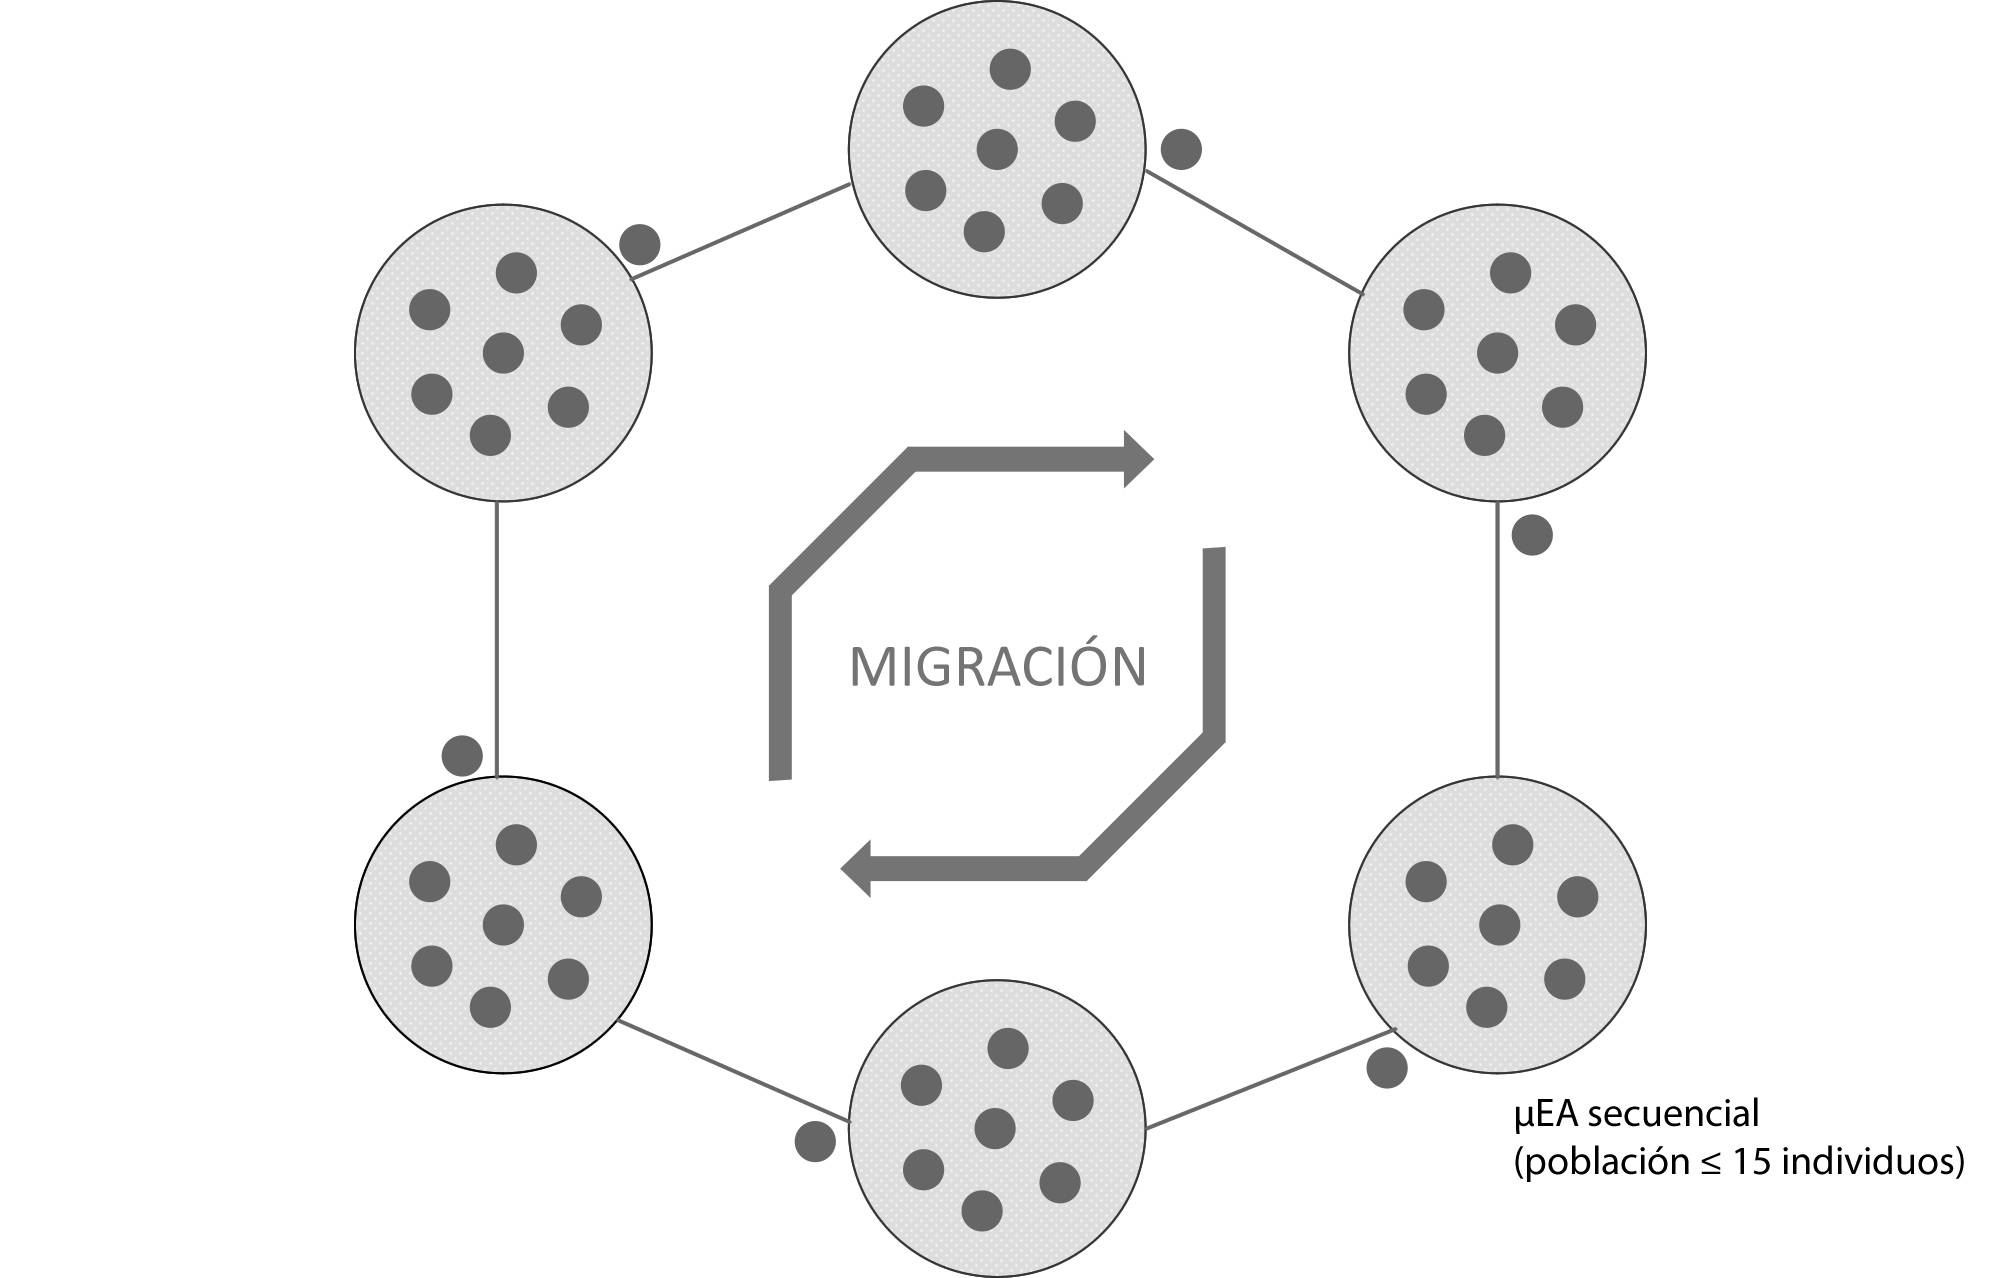
\includegraphics[width=.9\textwidth]{migracion.png}
\end{columns}
\end{block}

}

% ==============================================================


\section{Evaluación experimental}
\frame{\frametitle{Algoritmo ávido}
Bla bla bla...
\includegraphics[width=1.\linewidth]<1>{greedy_costo_1}
\includegraphics[width=1.\linewidth]<2>{greedy_costo_2}
\includegraphics[width=1.\linewidth]<3>{greedy_costo_3}
\includegraphics[width=1.\linewidth]<4>{greedy_costo_4}
\includegraphics[width=1.\linewidth]<5>{greedy_costo_5}
\includegraphics[width=1.\linewidth]<6>{greedy_costo_6}
\includegraphics[width=1.\linewidth]<7>{greedy_costo_7}
\includegraphics[width=1.\linewidth]<8>{greedy_costo_8}
}


% Slide 1 ==============================================================

\section{Introducción}
\frame{\tableofcontents[currentsection]}

\frame{
	\frametitle{Motivación} 
	\begin{block}{Car pooling}
		\begin{itemize}
			\item Beneficios en el plano ecológico y económico, individuales y colectivos.
			\item Diferentes iniciativas para atender el interés del público: carriles exclusivos, campañas para compartir los viajes al trabajo y aplicaciones para encontrar compañeros de viaje.
		\end{itemize}
	\end{block}
	
	\pause %Pausa entre bloques
	
	\begin{block}{Taxi pooling}
		\begin{itemize}
			\item Los taxis son un medio de transporte rápido y confiable, especialmente en ciudades donde el transporte público es poco eficiente.
			\item Los taxis raramente viajan a capacidad completa, impactando en la congestión del tráfico y en la contaminación de las ciudades.
			\item Tarifas altas desalientan a los usuarios.
			\item \alert{15\%} de los accidentes fatales en Uruguay involucran a un conductor alcoholizado (UNASEV).
	\end{itemize}
	\end{block}
}


% Slide 2 ==============================================================

\section{Definición del problema} 
\frame{\tableofcontents[currentsection]}

\frame{
	\frametitle{Descripción del problema}
	\begin{block}{Realidad estudiada}
Un grupo de personas ubicadas en un \textbf{mismo lugar de origen}, desean viajar hacia \textbf{diferentes destinos} utilizando taxis de forma compartida.

Se busca determinar la cantidad de taxis, la asignación de pasajeros y las rutas a seguir, de forma de \alert{minimizar el costo total del grupo de pasajeros}.
	\end{block}
\pause
	\begin{block}{Consideraciones}
		\begin{itemize}
			\item Cada taxi puede trasladar a un número limitado de pasajeros.\pause
			\item El número máximo de taxis para $N$ pasajeros es $N$, en el caso particular de que cada pasajero viaje en un vehículo separado.\pause
			\item El costo de un taxi está dado por la suma del \textbf{costo inicial} (“bajada de bandera”) más el \textbf{costo determinado por la distancia} recorrida desde el origen hasta el destino final, pasando por cada uno de los destinos intermedios.\pause
			\item No se consideran otros posibles costos (e.g. esperas, propinas, peajes).
		\end{itemize}		
	\end{block}
}	


% Slide 3 ==============================================================					
\frame{
	\frametitle{Descripción del problema}
	\begin{block}{Formulación matemática}
		Dados:
		\begin{itemize}
			\item $P = \{p_1,p_2,\ldots,p_N\}$ conjunto de pasajeros que parten de $O$ y se trasladan a $D = \{d_1,d_2,\ldots,d_N\}$. \pause
			\item Una función $dest: P \rightarrow D$ que establece el destino de cada uno de los pasajeros.\pause
			\item Un conjunto de taxis $T = \{t_1,t_2,\ldots,t_M\}$; con $M \leq N$; y una función $C:T\rightarrow\{0,1,\ldots,C_{MAX}\}$ que indica la cantidad de pasajeros que viajan cada taxi. $C_{MAX}$ es la capacidad máxima permitida en un mismo taxi.\pause
			\item una constante $B$ que indica el costo inicial del taxi.\pause
			\item una función de distancia, $dist: \lbrace \lbrace O \rbrace \cup D \rbrace \times D \rightarrow \mathbb{R}^+_0$.\pause
			\item una función de costo $cost: \mathbb{R}^+_0 \rightarrow \mathbb{R}^+_0$.
		\end{itemize}
	\end{block}
}	


% Slide 4 ==============================================================					
\frame{
	\frametitle{Descripción del problema}
	\begin{block}{Formulación matemática}
		El problema consiste en hallar una planificación, es decir una función $f:P \rightarrow T \times \lbrace 1, \ldots,C_{MAX} \rbrace$ para transportar los $N$ pasajeros en $K$ taxis ($K \leq N$) que determine la asignación de pasajeros a taxis y el orden en que serán trasladados a los respectivos destinos, minimizando la función de costo total ($CT$) de la asignación, dada en la Ecuación~\ref{Eq:total_cost_mono}, donde $f^{-1}(t_i,j)$ indica el pasajero asignado a la posición $j$ (orden de traslado) en el taxi $t_{i}$ y $dest\big(f^{-1}(t_{i},0)\big)=O ,\;  \forall \: t_{i}$.

		\begin{equation}
			\label{Eq:total_cost_mono}
			CT  =  \sum\limits_{t_{i}, C(t_{i})\neq0} \Bigg[B+\sum\limits_{j=1}^{C(t_{i})}cost\bigg(dist \underbrace{\Big(dest\big(f^{-1}(t_{i},j-1)\big),des	\big(f^{-1}(t_{i},j)\big)\Big)}_{\text{destinos consecutivos en el recorrido del taxi } t_i}\bigg)\Bigg]
		\end{equation}
	\end{block}
}


% Slide 5 ==============================================================

\section{Algoritmos Evolutivos} 
\frame{\tableofcontents[currentsection]}

\frame{
	\frametitle{Algoritmos Evolutivos}

}


% Slide 6 ==============================================================

\section{Trabajo relacionado} 
\frame{\tableofcontents[currentsection]}

\frame{
	\frametitle{Trabajo relacionado}

}


% Slide 7 ==============================================================

\section{Implementación} 
\frame{\tableofcontents[currentsection]}

\frame{
	\frametitle{Implementación}

}




%%%% ================ Slide 8 - Evaluación Experimental ================ %%%%
% Slide 8.1 ==============================================================

\section{Evaluación experimental} 
\frame{\tableofcontents[currentsection]}

\frame{
	\frametitle{Evaluación experimental}
	
	\begin{block}{Generación de puntos realistas en el mapa}
		Para la generación de instancias realistas del problema se utilizó una herramienta presentada en el trabajo relacionado de Ma et al. llamada Generador de Pedidos de Taxis (\textit{Taxi Query Generator, TQG}).
	\end{block}

}

% Slide 8.2 ==============================================================
\frame{
	\frametitle{Evaluación experimental}

}

% Slide 8.3 ==============================================================
\frame{
	\frametitle{Evaluación experimental}

}

% Slide 8.4 ==============================================================
\frame{
	\frametitle{Evaluación experimental}

}

% Slide 8.5 ==============================================================
\frame{
	\frametitle{Evaluación experimental}

}

% Slide 8.6 ==============================================================
\frame{
	\frametitle{Evaluación experimental}

}

% Slide 8.7 ==============================================================
\frame{
	\frametitle{Evaluación experimental}

}

% Slide 8.8 ==============================================================
\frame{
	\frametitle{Evaluación experimental}

}


% Slide 9 ==============================================================

\section{Planificador de viajes compartidos en línea} 
\frame{\tableofcontents[currentsection]}

\frame{
	\frametitle{Planificador de viajes compartidos en línea}

}


% Slide 9 ==============================================================

\section{Conclusiones y trabajo futuro} 
\frame{\tableofcontents[currentsection]}

\frame{
	\frametitle{Conclusiones y trabajo futuro}

}

\end{document}\grid